% !TEX TS-program = pdflatex
% !TEX encoding = UTF-8 Unicode

% This file is a template using the "beamer" package to create slides for a talk or presentation
% - Introducing another speaker.
% - Talk length is about 2min.
% - Style is ornate.

% MODIFIED by Jonathan Kew, 2008-07-06
% The header comments and encoding in this file were modified for inclusion with TeXworks.
% The content is otherwise unchanged from the original distributed with the beamer package.

\documentclass{beamer}
\usetheme{metropolis}

\AtBeginSection[]{
  \begin{frame}
  \vfill
  \centering
    \begin{beamercolorbox}[sep=8pt,center,shadow=true,rounded=true]{title}
    \usebeamerfont{title}
    \insertsectionhead\par%
    \end{beamercolorbox}
  \vfill
  \end{frame}
}


% Copyright 2004 by Till Tantau <tantau@users.sourceforge.net>.
%
% In principle, this file can be redistributed and/or modified under
% the terms of the GNU Public License, version 2.
%
% However, this file is supposed to be a template to be modified
% for your own needs. For this reason, if you use this file as a
% template and not specifically distribute it as part of a another
% package/program, the author grants the extra permission to freely
% copy and  modify this file as you see fit and even to delete this
% copyright notice. 


%\setbeamertemplate{background canvas}[vertical shading][bottom=white,top=structure.fg!25]
% or whatever


%\setbeamertemplate{headline}{}
%\setbeamertemplate{footline}{}
%\setbeamersize{text margin left=0.5cm}
  
\usepackage[english]{babel}
% or whatever

\usepackage[utf8]{inputenc}
% or whatever

\usepackage{times}
\usepackage[T1]{fontenc}
% Or whatever. Note that the encoding and the font should match. If T1
% does not look nice, try deleting the line with the fontenc.





\title[Discrete Math]{A Short Course in Discrtete Mathematics for the Computer Science Undergraduate}
\author{Dale Fletter}
\institute{UC Davis, ECS20, Summer Session 2}
\date{}

\usepackage{graphicx} % support the \includegraphics command and options
\usepackage {graphics}
\graphicspath{ {../../Outline-tex/illustrations/} }

\begin{document}
\begin{frame}
\titlepage
\end{frame}

\section{Proofs}

\begin{frame}{The Language of Formal Mathematics}
A prerequisite to this course is prior experience to the axiomatic method which is generally taught in high school geometry, also called deductive logic. Here is a summary of the key terms:
\begin{itemize}
\item Axiom or Postulate
\item Proof
\item Rules of Inference
\end{itemize}
\end{frame}

\begin{frame}
A proof is an \textit{argument} which contains some series of statements meant to convince the reader of the truth of some proposition we call the \textit{conclusion}.
\end{frame}

\begin{frame}
An argument in propositional logic is a sequence of propositions. All but the final proposition in the argument are called premises and the final proposition is called the conclusion. An argument is valid if the truth of all its premises implies that the conclusion is true.

An argument form in proposition logic is a sequence of compound propositions involving propositional variables. An arguent form is valid if no matter which particular propositions are substituted for the proposition variables in its premise, th econclusion is true if the premises are all true. (valid v sound??)
\end{frame}

\begin{frame}
A sentence whose symbolic translation is a tautology may be used at any time in a proof.
\end{frame}

\begin{frame}
The propositional statement
$$p \land (p \rightarrow q) \rightarrow q$$
is a tautology.
\end{frame}

\begin{frame}
We can string propositions together but it is common in some presentations of an argument to use separate lines like this:\\
\begin{tabular}{l|ll}
1 & R &Assumption 1 \\
2 & S & . \\
. & . &.\\
. & . &.\\
. & . &.\\
\hline
n & Conclusion & Justification \\
\end{tabular}\\
This is called a two-column presentation and is helpful when first learning to make formal arguments. It ensures you can cite the exact rule of inference applied to make the new assertion.
\end{frame}

\begin{frame}
\begin{table}[htbp]
   \centering
   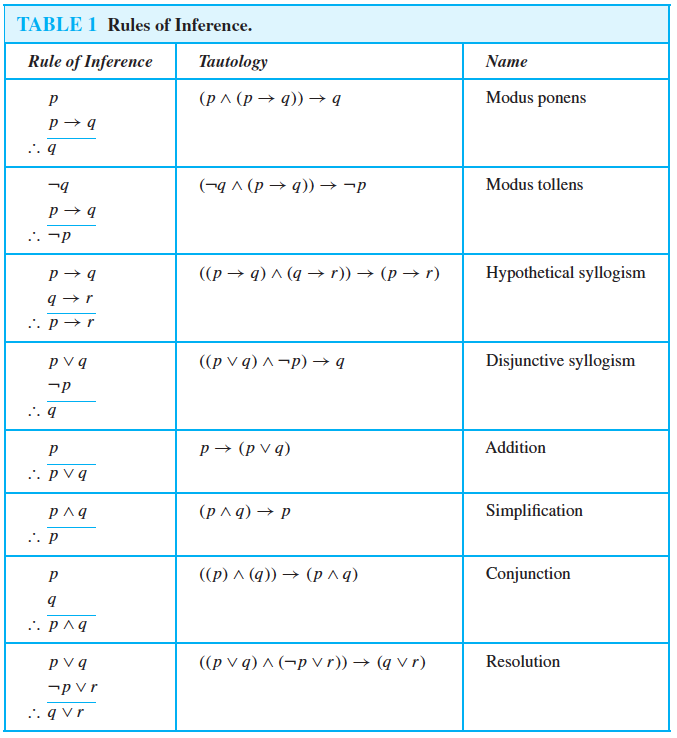
\includegraphics [width=3in] {Table-1-6-1-RulesOfInference}
   \caption{Common Rules of Inference}
   \label{table:rulesofinference}
   \end{table}
\end{frame}
 

\begin{frame}
You are at a crime scene and established the following facts:
\begin{itemize}
\item If the crime did not take place in the \textbf{B}illiar room, then Colonel \textbf{M}ustard is guilty.
\item The \textbf{L}ead pipe is not the weapon.
\item Either Colonel Mustard is not guilty or the weapon used was a lead pipe.
\end{itemize}
\end{frame}

\begin{frame}
\begin{tabular}{l|ll}
 1 & $\neg B \implies M$ &premise \\
2 & $\neg L$ & premise \\
3 & $\neg M \lor L$ &premise\\
4 & $\neg M$ & Disj Syl,2,3\\
\hline
 5 &$\therefore$ B & Contra 1,5\\
\end{tabular}\\
\end{frame}

\begin{frame}
Any valid proof must be capable of decomposing into this basic two-column form if needed.
\end{frame}

\begin{frame}{Direct Proof}
PROVE $P \implies Q$
\begin{proof}
\begin{tabular}{l|ll}
& Assume P.& \\
 &\vdots& \\
 & Therefore Q.&  \\
 & Thus, $P \implies Q $&\\

\end{tabular}\\
\end{proof}
\end{frame}


\begin{frame}{Definition of Even and Odd Integers}
An even integer is one that is equal to twice some other integer. An odd integer is one that is equal to twice some other integer plus 1.
\end{frame}

\begin{frame}
Prove: If $x$ is an odd integer, then $x+1$ is even.
\begin{proof}
Let $x$ be an integer and suppose $x$ is odd. (This is the antecedent of the conditional. Now we must derive `$x+1$ is even'.) Since $x$ is odd, it can be restated as $2k+1$ where $k$ is some integer, in other words $x=2k+1$ (the definition of odd). $x+1=(2k+1)+1$ (adding equals to equals gives equals). $x+1=2k+2$. $x+1=2(k+1)$. $x+1$ is twice some other integer. Therefore, $x+1$ is even by the definition of an even integer. This is the conclusion we set out to achieve or  QED.
\end{proof}
\end{frame}

\begin{frame}
This last example was in the prose style of proof presentation, the one that is generally used for proofs in this and subsequent math courses.
\end{frame}




\begin{frame}{Another Example of Direct Proof}
Given that for all positive integers $n$, if $n$ is greater than 4, then $n^2$ is less than $2^n$, prove that $100^2 < 2^{100}$.
\begin{proof}
Let $P(n)$ denote "$n>4$" and let $Q(n)$ denote "$n^2$". The statement "For all positive integers $n$, if $n$ is greater than 4, then $n^2$ is less than $2^n$ can be represented by $\forall n(P(n) \rightarrow Q(n)$, where the domain consists of all positive integers. We start by assuming that $\forall n(P(n) \rightarrow Q(n)$ is true. Note that $P(100)$ is true because $100 > 4$. It follows by universal modus ponens that $Q(n)$ is true, namely that $100^2 < 2^{100}$. 
\end{proof}
\end{frame}

\begin{frame}{Proof by Cases}
Sometimes a single direct proof is not possible but two or more together are sufficient.
PROVE: $(P \lor Q) \implies R$
\begin{proof}
$(P \lor Q) \implies R \equiv (P\implies R) \lor (Q \implies R)$ 
CASE 1: PROVE: $P\implies R$
  Assume $P$.\\
  \vdots
  Therefore $R$. Thus $P\implies R$.\\


CASE 2: PROVE: $Q \implies R$.\\
  Assume $Q$.\\
  \vdots 
  Therefore $R$. Thus $Q\implies R$.\\

Thus $(P \implies R) \lor (Q \implies R)$
\end{proof}
\end{frame}

\begin{frame}{Proof by Contraposition}
Recall that $P\implies Q \equiv \neg Q \implies \neg P$.
This tells you that if you cannot prove that $P \implies Q$ you should attempt to prove that $\neg Q \implies \neg P$. 
\end{frame}

\begin{frame}{Proof by Contradiction}
Recall that $\neg T \equiv F$. This offers another stragegy for a proof. If instead of trying to do a direct proof, or if you cannot use direct proof, it is sometimes possible to assume the opposite of what you are given and show that it MUST yield a contradiction. Any proposition that leads to a contradiction is logically equivalent to a contradiction and that means that it MUST BE FALSE. If the opposite of the proposition given leads to a contradiction, the reverse must be true, that the given proposition is a tautology, that it MUST BE TRUE. Here is the most common example of proof by contradiction.
\end{frame}

\begin{frame}{The square root of 2 is irrational}

Note that the proposition is not a conditional statement so a direct proof is difficult. We try to prove using proof by contradiction. Assume that the square root of 2 is the opposite of irrational, that it is rational, that it can be stated as a fraction of two integers, $m$ and $n$ such that there are no common factors between them, that it is stated in lowest common terms. Then $m/n=\sqrt{2}$,  $2=m^2/n^2$ and $2n^2=m^2$. 

\end{frame}

\begin{frame}{The square root of 2 is irrational (contd)}
Since $m^2$ and $n^2$ contain an even number of factors (something you already know from high school but something we will prove in this course later), you know both must be even. Now consider the expression $2n^2$. It has an odd number of the factor 2. But we already know that $m^2$ must contain an even number of factors of 2. How can both things be true? They cannot. We have been led to a contradiction. If we have a contradiction we must reject the assumption we originally made which led to this, namely that the square root of 2 is rational. It's opposite is that the square root of two is IRrational since it must be one or the other (the principle of the excluded middle in logic). 
\end{frame}

\section{Proofs with Quantified Statements}
\begin{frame}
Some truths in mathematics have to do with the existence of a number with certain properties. One way to prove such a statement is to provide a number that satisfies the properties. These are existence theorems. These are also called constructive proofs since we construct the object needed to satisfy the condition.
\end{frame}

\begin{frame}
Prove `There is an even prime natural number.'
Proof. We are asked to prove the statement, `There exists a natural number $n$ such that $n$ is prime and $n$ is even. The number 2 is prime and it is even. QED.
\end{frame}

\begin{frame}
Some constructive proofs are very difficult \dots .
\end{frame}

\begin{frame}
Prove there exists a  natural number whose fourth power is the sum of three other fourth powers.
Proof. 20615673 is such a number since it is equal to the sum $2682440^4+15365639^4+18796760^4$. QED.
\end{frame}

\begin{frame}
Just as a point of curiosity, there are some proofs which are non-constructive existence proofs. They show that a number of the type must exist but do not provide a way to finding such a number. We will see an example in a later chapter.
\end{frame}

\begin{frame}
Sometimes we need to prove that something is true over the entire domain of discourse. This is a form of universal instantiation. Sometimes it is difficult to see in the statement that the proof is for all objects in the domain.
\end{frame}

\begin{frame}
Prove that if $n$ is an even integer, then $n^2$ is an even integer.
Proof. The conditional is of the form, $\forall n P(n)$ where the universe is integers and $P$ is the predicate, `If $n$ is even, then $n^2$ is even.' Note that the choice of $n$ from the universe is arbitrary. This fixes the $n$ and we proceed as a direct proof by assuming the antecedent. The rest follows from the definition of even. QED.
\end{frame}

\begin{frame}
The reason the prior proof is a proof of the universal truth for all integers is because the choice of the particular $n$ was arbitrary.
\end{frame}

\begin{frame}{Proving a Universal by Contradiction}
Prove $\forall x P(x)$.
Proof. Let us assume the opposite, that $\neg \forall x P(x)$. Then $\exists \neg P(x)$. We are now allowed to assume that there is an object $t$ such that $\neg P(t)$ is true. This leads to a contradiction of $Q \land \neg Q$. We must then reject the assumption as also false and affirm the opposite that for all $x$ in the domain that for any $x P(x)$. \\

Following is a list of the important rules of inference that can be used with quantified statements.
\end{frame}


\begin{frame}
\begin{table}[htbp]
  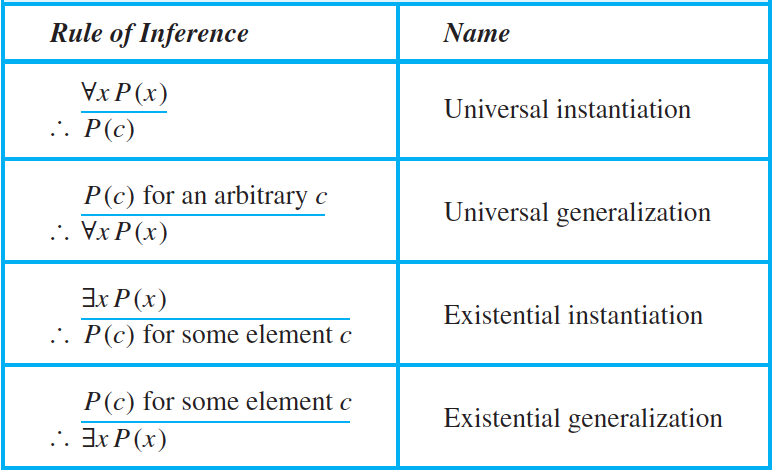
\includegraphics [width=3in]
  {Table-1-6-2-RulesOfInferenceForQuantifiedStatements}
  \caption{RulesOfInferenceForQuantifiedStatements}
  \label{table:RulesOfInferenceForQuantifiedStatements}
  \end{table}
\end{frame}




\end{document}


